% !TEX root = ../VPJ.tex

\chapter{Schnittstelle zum Robotino}
\label{sec:Schnittstellen}

%\section{Kommunikation zu Robotinos}
\label{sec:Gewerk2Protokoll}

Die Robotinos werden von Gewerk 2 verwaltet und programmiert. Um eine erfolgreiche Kommunikation zwischen Fertigungsplanungsrechner und Robotino zu gewährleisten existieren folgende Vereinbarungen mit Gewerk 2.

Die Kommunikation geschieht über UDP. Da UDP ein verbindungsloses Protokoll ist muss nicht sichergestellt werden dass Robotino oder Fertigungsplanungsrechner immer verbunden sind. Die Nachrichten werden an spezifizierten Ports gesendet und empfangen.

Die in Tabelle \ref{tab:Ports} dargestellte Vereinbarung wurde für die Ports getroffen.

\begin{table}[!ht]
	\centering
	\begin{tabular}{|c|c|c|}
		\hline
		Roboter IP Adresse & Sendeport &	Empfangsport \\
		\hline
		192.168.0.11 & 25010 & 25011 \\
    192.168.0.12 & 25020 & 25012 \\
    192.168.0.13 & 25030 & 25013 \\
    192.168.0.14 & 25040 & 25014 \\
    192.168.0.25 & 25050 & 25015 \\
		\hline
	\end{tabular}
	\caption{Portvereinbarung}
	\label{tab:Ports}
\end{table}

\section{Sequenzdiagramm}
\label{sec:sequenzdiagram}

Zunächst wurde eine Struktur entwickelt, in der beschrieben wird, wie die Daten zwischen Robotino und Fertigungsplanungsrechner ausgetauscht werden sollen. Dies wurde anschließend in einem Sequenzdiagramm, Abbildung \ref{fig:Sequenzdiagramm}, dargestellt. 

\begin{figure}[htb]
    \centering
    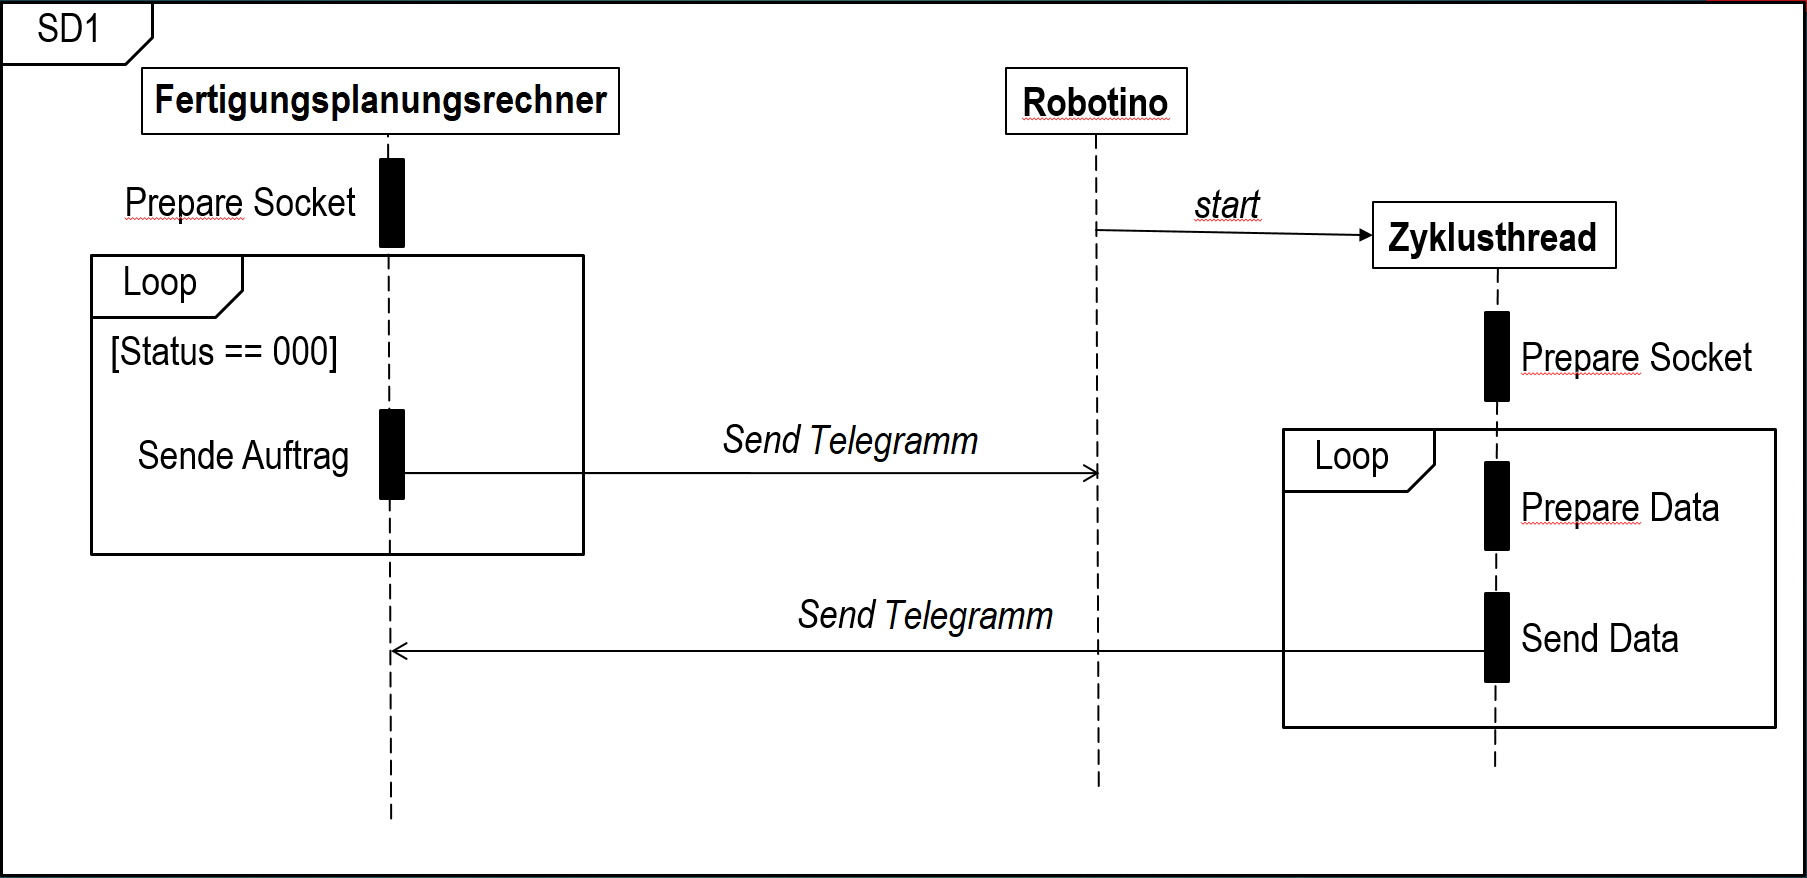
\includegraphics[width=0.9\textwidth]{Abbildungen/Sequenzdiagramm.PNG}
    \caption{Sequenzdiagramm}		
    \label{fig:Sequenzdiagramm}
\end{figure}

Dem Sequenzdiagramm ist zu entnehmen, dass der Robotino nach Programmstart zyklisch Daten sendet. Die Zykluszeit beträgt 100 ms. Da die Daten über UDP an einen spezifizierten Port versendet werden ist ein Empfänger nicht zwangsweise erforderlich und die Programme können unabhängig voneinander laufen. Der Inhalt der Daten ist in Abschnitt \ref{sec:Telegramme} beschrieben. Solange der Robotino läuft werden die Daten gesendet. Dadurch kann auch ein Ausfall der Kommunikation festgestellt werden. 

Auf Seiten des Fertigungsplanungsrechners wird nur bei Bedarf ein Sendevorgang eingeleitet. Erst wenn ein Auftrag an den Robotino gesendet werden soll wird eine Schleife ausgeführt. In der Schleife wird der Auftrag zyklisch an den Robotino gesendet. Die Zykluszeit beträgt hierbei 700 ms. In Kapitel \ref{sec:StateMachineImplementierung} ist die in einer State-Machine implementierte Schleife beschrieben. Die Schleife kann durch Empfangen einer Statusänderung des Robotinos verlassen werden. Dadurch wird eine erfolgreiche Übertragung des Auftrags sichergestellt werden. Die im Auftrag befindlichen Daten sind in Abschnitt \ref{sec:Telegramme} näher erläutert.

\section{Telegramme}
\label{sec:Telegramme}

Die Telegramme zwischen Robotino und Fertigungsplanungsrechner bestehen aus einer festgelegten Struktur. Dabei ist sowohl die Länge der Telegramme als auch der Inhalt festgeschrieben. In beiden Telegrammen werden Double-Werte in einem Byte versendet. Jedes Byte muss daher kodiert und dekodiert werden. 

\subsection{Telegramm vom Fertigungsplanungsrechner zu Gewerk 2}

Der Auftrag, der an den Robotino gesendet wird, enthält 5 Bytes. Eine Aufschlüsselung ist in Tabelle \ref{tab:TelegrammZuG2} dargestellt. 

\begin{table}[!ht]
	\centering
	\begin{tabular}{|r|c|l|}
		\hline
		Byte & Inhalt	&	Beschreibung \\
		\hline
			1  & Auftragsart & 1: Transport; 2: Parken; 3: Laden  \\
			2  & Position 1  & z.B. 11 \\
			3  & Position 2  & z.B. 32 \\
		  4  & AliveStatus & 1 senden nach Alive Anfrage \\
		  5  & *Reserved   &  \\
		\hline
	\end{tabular}
	\caption{Telegramm zu Gewerk 2}
	\label{tab:TelegrammZuG2}
\end{table}

Das erste Byte klassifiziert die Auftragsart. Diese beschreibt, welche Tätigkeit der Robotino als nächstes tun soll. Auftragsart eins bedeutet, dass der Robotino einen Transportauftrag erhalten hat, also ein Werkstück von einer Position zu einer anderen \Gls{Position} fahren soll. Die Auftragsart 2 zeigt an, dass der Robotino auf einen Parkplatz geschickt wird. Eine Ladefahrt wird mit Auftragsart 3 gekennzeichnet. 

Im zweiten und dritten Byte sind die Positionen angegeben, an welche sich der Robotino bewegen soll. Dabei wird Position 2 nur bei Auftragsart 1 befüllt bzw. ausgewertet, da ein Parken und Laden nur eine Zielposition benötigt. Bei Auftragsart 1 jedoch zeigt Position 1 den Arbeitsplatz an, wo das Werkstück abgeholt werden soll und Position 2 den Ablageort des Werkstücks. 

Über das vierte Byte kann dem Robotino ein Status-Flag gesendet werden. Sobald der Robotino eine Anfrage zu dem Flag sendet wird eine 1 zurückgesendet. Ansonsten ist der Wert 0. Damit kann der Robotino die Funktionalität der Kommunikation validieren.

Mit dem fünften Byte wird eine einfache Erweiterung des Telegramms ermöglicht, sofern mehr Daten übertragen werden sollen. Am Anfang der Ausarbeitung des Projektes war das vierte Byte ebenfalls ein reserviertes Byte. 

Um Robotino 5 mit einzubinden wurde mit Gewerk 4 eine Sonderform des Protokolls vereinbart. Die Vereinbarung sieht vor, die Auftragsart zum starten der Ladefahrt auf 1 zu setzen, wobei die Position 1 die 06 ist. Alle weiteren Felder sollen mit 00 gefüllt werden. Um die Ladefahrt erneut starten zu können kann die Auftragsart auf 0 zurückgesetzt werden. 

\subsection{Positionskodierung}
\label{sec:Positionskodierung}

Aus den Positionen, die dem Robotino gesendet werden kann eindeutig bestimmt werden, an welchen Ort der Robotino fahren soll. 

Eine Aufschlüsselung der Positionen ist in Abbildung \ref{fig:Positionskodierung} dargestellt. Hier ist die Anordnung von Stationen, Parkplätzen und Ladestationen im Raum dargestellt, mitsamt ihrer Positionskodierung. 

\begin{figure}[htb]
    \centering
    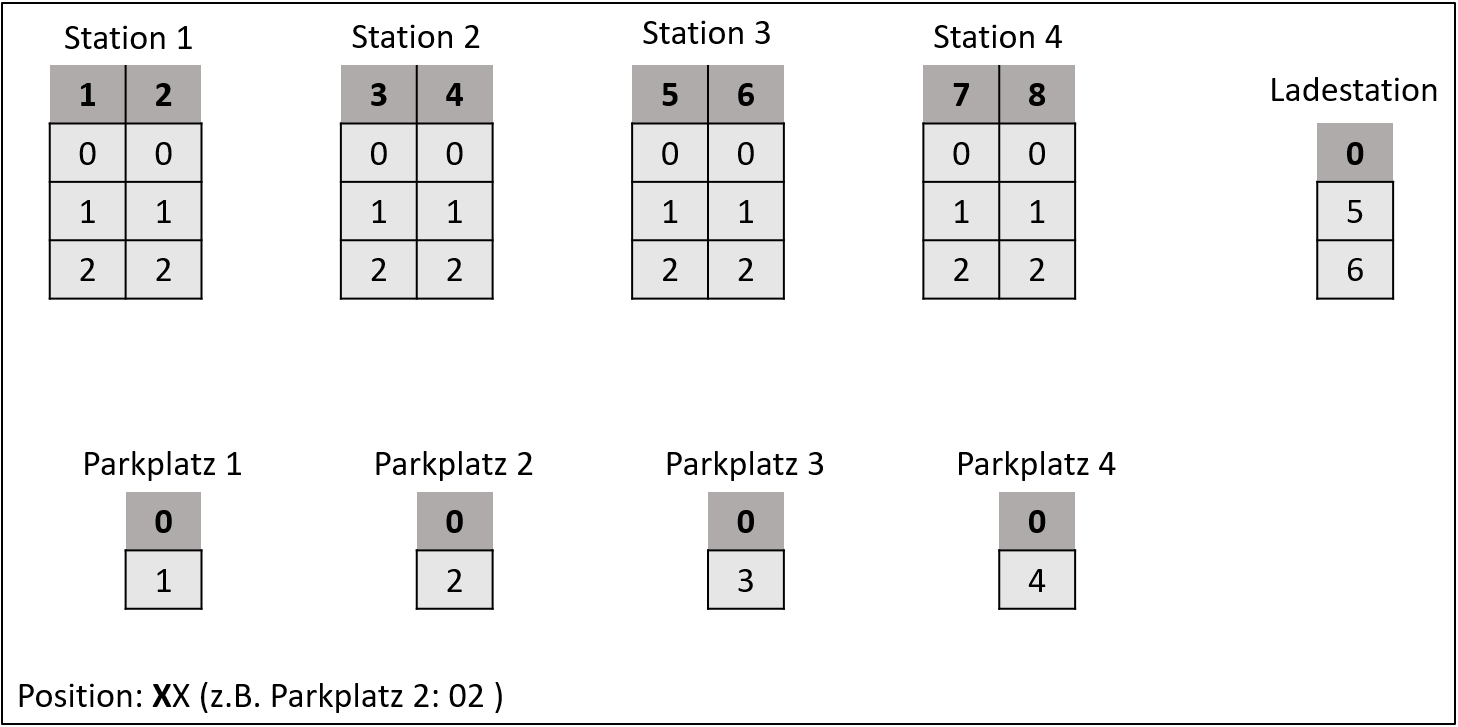
\includegraphics[width=0.9\textwidth]{Abbildungen/Positionskodierung.PNG}
    \caption{Positionskodierung}		
    \label{fig:Positionskodierung}
\end{figure}

Jede Position ist kodiert in einer Zahl bestehend aus zwei Ziffern. Die erste Ziffer beschreibt dabei die Stationsnummer aufsteigend von 1 bis 8. Parkplätze und Ladestationen haben als Kennung in der ersten Ziffer eine 0. 

Mit der zweiten Ziffer kann die genaue Position innerhalb einer Station spezifiziert werden. In den Stationen 1 bis 8 ist der RFID-Lesekopf mit Ziffer 0 und die Arbeitsplätze mit den Ziffern 1 und 2 kodiert. Die Parkplätze sind aufsteigend mit den Ziffern 1 bis 4 durchnummeriert. Hieran anschließend sind beide Ladestationen mit Ziffer 5 und 6 kodiert. 

So ergibt sich für Beispielsweise Parkplatz 2 eine Kodierung von 02, für die untere Ladestation die Kodierung 06 oder für den oberen Arbeitsplatz an Station 3 die Kodierung 31.

\subsection{Telegramm vom Robotino zum Fertigungsplanungsrechner}

Das zyklisch gesendete Telegramm vom Robotino enthält alle Informationen, die zur Auftragsgenerierung und Robotinoanzeige nötig sind. Alle Telegrammeinträge sind in Tabelle \ref{tab:TelegrammVonG2} dargestellt. Das Telegramm enthält neun Einträge, welche je einen Double-Wert enthalten. 

\begin{table}[!ht]
	\centering
	\begin{tabular}{|r|c|l|}
		\hline
		Byte & Inhalt	&	Beschreibung \\
		\hline
			1  & Error &  Errortyp  \\
			2  & Akku  & Prozentwert als Integer \\
			3  & Hindernis & Hindernistyp zwischen 00 und 03\\
		  4  & *Reserved &  interner Roboterstatus \\
		  5  & AliveAbfrage  & 1: Roboterabfrage erfordert Antwort; 0: egal \\
		  6  & Status & $X_1X_2X_3$; 000: nichts zu tun \\
		  7  & Greifer   & 0:leer; 1:voll \\
		  8  & *Reserved &  \\
		  9  & *Reserved   &  \\
		\hline
	\end{tabular}
	\caption{Telegramm von Gewerk 2}
	\label{tab:TelegrammVonG2}
\end{table}

Im ersten Byte sendet der Robotino einen Error. Die einzelnen Errortypen und die nötige Reaktion sind in Kapitel \ref{sec:Error} dargestellt. 

Aus dem zweiten Byte kann der aktuelle Akkustand des Robotinos gelesen werden. Dieser liegt zwischen 0, vollständig entladen, und 100, vollständig geladen. 

Über das dritte Byte kann gelesen werden, ob der Robotino ein Hindernis erkannt hat. Beim Empfangen einer 00 ist kein Hindernis im Weg und der Robotino kann sich normal bewegen. Eine Änderung des Wertes kann zunächst nur zu 03 erfolgen. Das bedeutet, der Robotino hat ein Hindernis erkannt, dieses aber noch nicht klassifiziert hat. Über die Zahl 01 wird kodiert, dass der Roboter ein Hindernis erkannt hat, dies aber nicht weiter Klassifizieren kann. Mit einer 02 wird angezeigt, dass das erkannte Hindernis ein anderer Robotino ist. Aufgrund der Umgebungsstörungen kann es sein, dass der Robotino immer wieder abwechselnd eine 00 und eine 01 sendet. 

Das vierte Byte wird von Gewerk 2 für eine interne Bekanntmachung verschiedener Roboterstati genutzt. Der Wert wird nicht versendet und bleibt immer 0.

Über das fünfte Byte kann der Robotino eine Anfrage triggern. Sobald eine 1 empfangen wird, so wird im nächsten Telegramm an den Robotino der AliveStatus zu eins gesetzt. Dadurch kann der Robotino validieren, dass die Kommunikation noch vorhanden ist. Ansonsten ist der Wert 0. 

Mit dem sechsten Byte wird der aktuelle Roboterstatus kodiert. Dieser Wert ist für die Auftragsplanung am wichtigsten. Die Zahl besteht immer aus drei Ziffern. Die erste Ziffer dient dabei als Typisierung des Status. Wenn der Status 000 ist, bedeutet das, der Robotino hat nichts zu tun und benötigt einen Auftrag. Auf einem Parkplatz wird keine 000 gesendet. Immer wenn ein Robotino neu eingesetzt wird, seinen aktuellen Transportauftrag abgeschlossen hat, aus einem Errorstatus kommt oder den Ladevorgang an der Lasestation abgeschlossen hat wird eine 000 gesendet. 

Wenn die erste Ziffer eine 1 ist, befindet sich der Robotino auf dem Weg zu einer Position. Bei einer 2 als erste Ziffer ist der Robotino gerade an einer bestimmten Position. Über den Wechsel von 1 auf 2 kann somit das Erreichen einer Position erkannt werden oder der Verlassen einer Position über den Wechsel auf 1. 

Die beiden letzten Ziffern des Status kodieren die Position in der in Abschnitt \ref{sec:Positionskodierung} beschriebenen Art. 

Das der Greifer des Robotinos geschlossen, also voll, ist wird im siebten Byte mit einer 1 angezeigt. Bei offenem Greifer ist der Wert 0.

Das achte und neunte Byte sind für einfache Erweiterung des Telegramms um weitere Informationen geplant gewesen. Bei Projektstart war das vierte und fünfte Byte ebenfalls reserviert, wurde aber während des Projekts zugewiesen. 

\section{Fehlertypen und Behebung}
\label{sec:Error}

Der Robotino kann über den Errorstatus verschiendene aufgetretene Fehler anzeigen. Drei dieser Fehlertypen und ihre Behandlung sind in den nächsten Abschnitten beschrieben. In Normalfall ist der Error 1. Das bedeutet es ist alles in Ordnung. 

\subsubsection{Fehlertyp 2}

Wenn der Fehlertyp 2 empfangen wurde, bedeutet das, der Robotino hat sein Werkstück verloren. Diese Meldung tritt genau dann auf, wenn der Greifer des Robotinos zwar geschlossen ist, die Lichtschranke jedoch ein Verlust des Werkstücks detektiert. 

Zur Behebung des Errors wird die Auftragsplanung pausiert und das verlorene Werkstück gesucht und aus der Fertigungsstraße entfernt. Anschließend wird der zugehörige Prozess geblockt. Die Zielstation des Robotinos wird per Hand freigegeben und eventuelle Reservierungen vom entfernten Werkstück aufgehoben. 

In der Praxis konnte dieser Fehler nur mit Gewalt hervorgerufen werden, da ein gegriffenes Werkstück sehr stark festgehalten wird und ein Verlust damit unwahrscheinlich ist. 

\subsubsection{Fehlertyp 3}

Wenn der Robotino einen Transportauftrag erhält und am Abholort kein Werkstück greifen kann wird Fehler 3 gesendet. 

Die Fehlerbehebung ist identisch zur Fehlerbehebung von Fehlertyp 2. Es muss erneut geprüft werden, welcher Prozess abgearbeitet werden sollte, und alle diesem Prozess zugeordneten Arbeitsplätze, Stationen o.ä. freigegeben werden. Der Auftrag muss blockiert werden.

Da die Auftragsvergabe die Position jedes Werkstück kennt, kann dieser Fehlerfall in der Praxis nur sehr selten aufgrund einer größeren Störung oder menschlichem Versagen auftreten. Ein möglicher Grund kann sein, dass der Robotino den Arbeitsplatz verfehlt hat oder das Werkstück von einem Anwender unbeabsichtigt entfernt wurde. 

\subsubsection{Fehlertyp 4}

Ein Fehler von Typ 4 bedeutet, dass keine Route planbar ist. In der Visualisierung muss je nach Situation bei auftreten des Fehlers verschieden reagiert werden. 

Wenn der Robotino direkt nach Erhalten eines Auftrags den Error sendet, kann der Auftrag direkt neu vergeben werden. 

Für den Fall, dass der Robotino inmitten eines Transportvorgangs eine Route nicht berechnen kann, muss im schlimmsten Fall der Robotino defekt geschalten werden. Im normalfall sollte der Robotino nachdem der Error auftrat die Route in bestimmten Zeitabständen versuchen neu zu berechnen, daher kann der Error zunächst nur beobachtet werden. Sollte der Robotino neu gestartet werden muss wie bei Fehlertyp 2 vorgegangen werden. 

Wenn der Robotino ohne einen Transportauftrag keine Route planen kann ist dies für die Auftragsplanung nur bedingt relevant und der Error kann als Info angesehen werden. 

